\section{Analog to Digital Converter}
\subsection{Discrete ADC Simulation}
The initial stage of the voice recording circuit is an analog to digital
converter allowing the digital storage system to process the analog input from
an eletret microphone.  A simplified ADC schematic was provided in the lab
instructions, and was simulated with Cadence PSpice as shown in
Figure~\ref{f:adc_schem}.
%
\begin{figure}[H]
\centering
	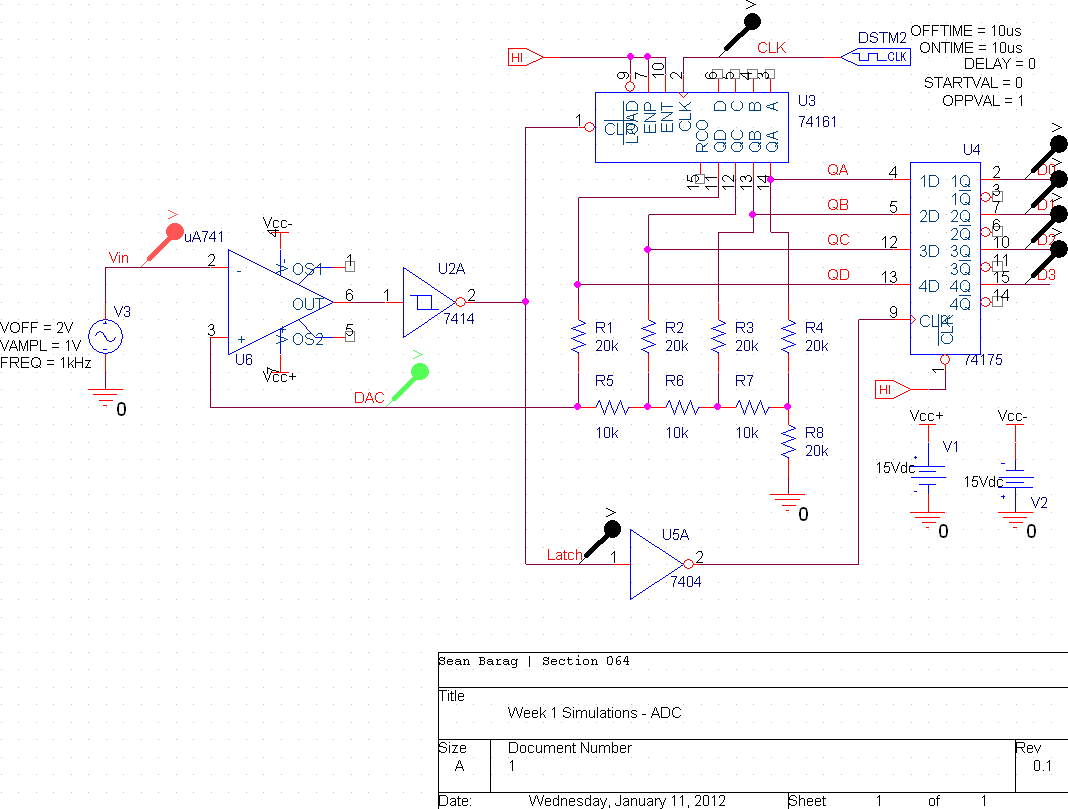
\includegraphics[width=.8\textwidth]{img/shot/part2_schem_cropped.PNG}
	\parbox{.8\textwidth}{
	\caption[Discrete ADC --- Schematic]{Schematic for the simplified ADC
	provided by the lab instructions.}
	\label{f:adc_schem}}
\end{figure}
%
This circuit was simulated using transient analysis lasting for
just~\SI{2}{\milli\second}.  Because of the~\SI{1}{\kilo\hertz} frequency of
the sinusoidal input signal, the system will be observed for two full input
periods, as shown in Figure~\ref{f:adc_plot}.

\subsection{Discrete ADC Results}
Upon the completion of the transient simulation, PSpice produced the plot
included in Figure~\ref{f:adc_plot}.
%
\begin{figure}[H]
\centering
	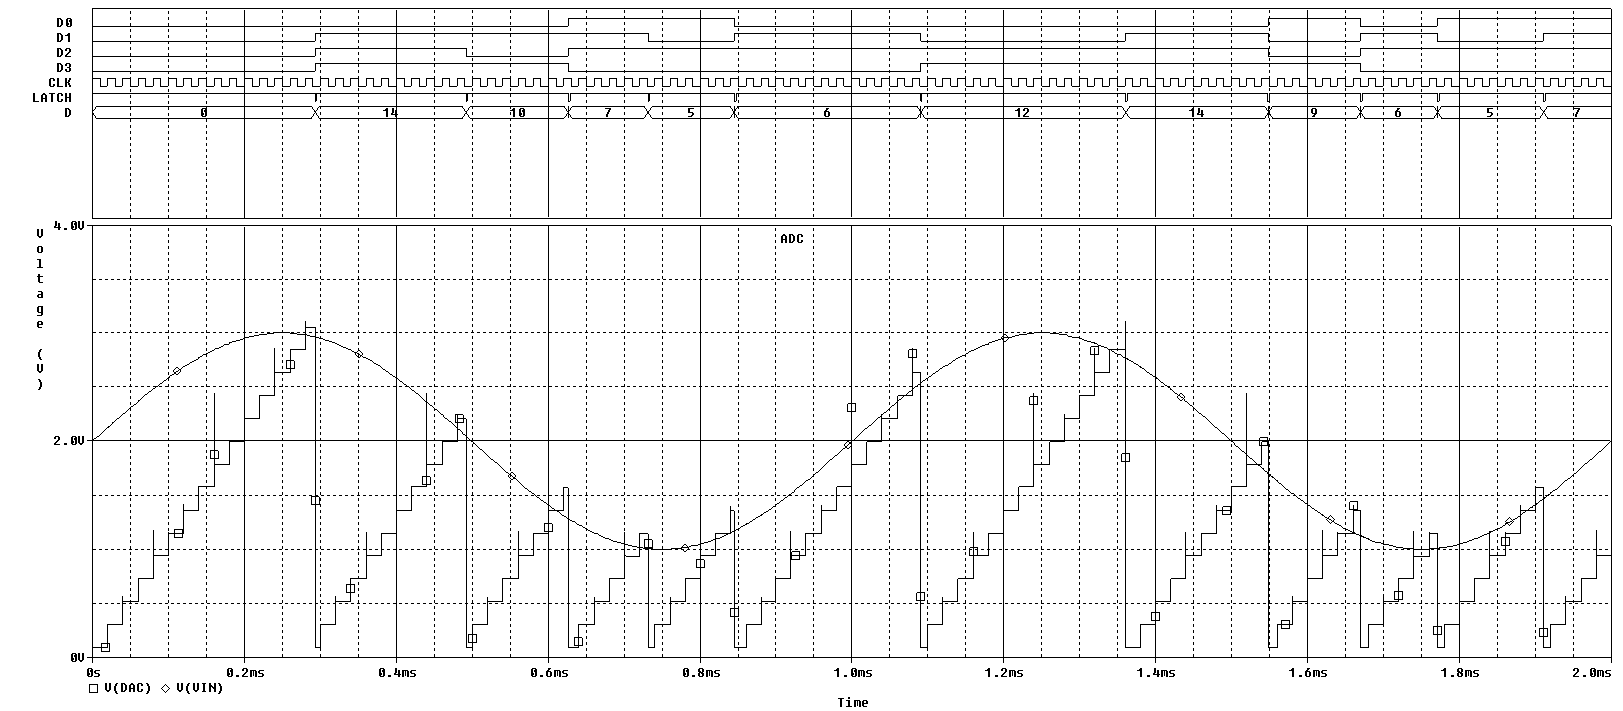
\includegraphics[width=.8\textwidth]{img/plot/part2_plot.PNG}
	\parbox{.8\textwidth}{
	\caption[Discrete ADC --- Results]{PSpice-produced plot of the input
	voltage and output voltages, as well as the voltages at the ``Latch'' and
	``Clk'' nodes as indicated above.  \textbf{Note that the schematic
	numbering in this schematic does not match the numbering from the lab
	instructions.  All numbering in this document refers to the elements in the
	included schematics.}}
	\label{f:adc_plot}}
\end{figure}
%
The plot reveals a lot of information about the function of this particular
ADC.  The value of the DAC line increases in discrete steps due to the binary
counter U3.  When the voltage on this line exceeds the input voltage, the latch
line goes low and triggers the D flip-flop U4 --- here acting as a buffer to
produce a steady output while the next set of bits is calculated --- to output
the corresponding digital bits D0 through D3 from its inputs.  At this time the
counter resets, latch goes high, and the counting process repeats.  While this
does provide accurate digital representations of individual signals, it causes
the rate of measurement to increase (and thus the resolution to decrease) for
inputs with larger voltages, as each value in the count up process is analyzed
for one clock period (in this case~\SI{20}{\micro\second}).

The block of resistors R1 through R8 acts as an R-2R network.  In this
configuration, each junction acts as a voltage divider, allowing exactly
half of the voltage at one node to appear at the next.  Thus each pin from the
binary counter U3 contributes a portion of voltage consistent with a binary
value,  i.e. the contribution of DA is twice as large as DB, which is twice as
large as DC, etc.  Since the sum of these voltages appears at the positive
input of U6, the opamp acts as a comparator, setting its output high when the
counter exceeds the system's input.
